%; whizzy-master "main.tex"

\chapter{Tutorial}\label{chap:tutorial}

\begin{target}beginners.\end{target}

This chapter aims at helping a developer to write their first \framac plug-in.
At the end of the tutorial, any developer should be able to extend \framac with
a simple analysis available as a \framac plug-in. This chapter was written as a
step-by-step explanation on how to proceed towards this goal. It will get you
started, but it does not tell the whole story. You will get it with your own
experiments, and by reading the other chapters of this guide as needed.

Section~\ref{tut2:environment} provides some tips for setting up a
development environment for \framac.
Section~\ref{tut2:architecture} shows what a plug-in looks like. Then
Section~\ref{tut2:hello} explains the basis for writing a standard \framac
plug-in\index{Plug-in}, while Section \ref{tut2:cfg} details how to interact
with \framac and other plug-ins to implement analyzers of \C programs.

\section{Development Environment}\label{tut2:environment}

It is easy to develop a plug-in for \framac with any IDE, as long as it
supports the OCaml language. This includes (but is not limited to)
Emacs or Vim with the Merlin\footnote{\url{https://ocaml.github.io/merlin}}
tool, or VS~Code with the {\em OCaml platform} extension.
The last is probably the easiest to setup for a beginner in OCaml.

Most modern IDEs support (directly or indirectly, via Merlin)
OCaml-LSP\footnote{\url{https://github.com/ocaml/ocaml-lsp}},
which is an implementation of LSP ({\em Language Server Protocol}) for OCaml.

Concerning code formatting, the \framac team currently uses the
\texttt{ocp-indent} opam package for code indentation.
Consider installing it if you want to ensure your code follows the same
conventions.

Overall, it is \textbf{strongly} suggested to use an OCaml-aware IDE and take
the time to set it up. Plug-ins use several different parts of the \framac API,
and a properly setup IDE greatly improves productivity, offering features such
as auto-completion, type checking, syntax highlighting, and code navigation.

\section{What Does a Plug-in Look Like?}\label{tut2:architecture}
\index{Plug-in!Architecture}\index{Architecture!Plug-in}

Figure~\ref{fig:overview} shows how a plug-in can integrate with the \framac
platform. This tutorial focuses on specific parts of this figure.

\begin{figure}[ht]
\begin{center}
\newsavebox{\designbox}
\savebox{\designbox}{\begin{varwidth}{\textwidth}\centering Design\\(GUI extension point)\end{varwidth}}
\newlength{\designheight}
\setlength{\designheight}{\totalheightof{\usebox\designbox}}
\newsavebox{\capbox}\savebox{\capbox}{\textbf{Caption:}}
\newlength{\captionheight}\settototalheight{\captionheight}{\capbox}
\begin{tikzpicture}[remember picture,txt/.style={inner xsep=3pt}]
  \node[inner sep=0pt] (implem) {
    \tikztitleboxbig{Plug-in\\implementation}{darkgreen}{
      \begin{tikz-vbox}{plugin-text}
        \node[on chain, draw, txt,minimum height=\designheight](register){Register};
        \node[on chain, draw, txt,minimum height=\designheight](options){Options};
        \node[on chain]{
          \begin{tikz-hbox}[every node/.style={minimum height=\designheight,minimum width=\designheight}]{etc-text}
            \node[draw, on chain]{};
            \node[on chain] {\ldots};
            \node[draw, on chain] {};
          \end{tikz-hbox}
        };
      \end{tikz-vbox}
    }
  };
  \node[anchor=south west,inner sep=0pt,xshift=\padding]
    at (implem.south east) (gui){
    \tikztitleboxbig{Plug-in GUI}{darkgreen}{
      \begin{tikz-hbox}{pluginguicontent}
        \begin{scope}[
          every node/.style={
            on chain,
            minimum width=\designheight,
            minimum height=\designheight}]
          \node[draw] {}; \node {\ldots}; \node[draw] {};
        \end{scope}
      \end{tikz-hbox}
    }
  };

  \coordinate[yshift=\padding] (dune-se) at (gui.north east);
  \coordinate (dune-nw) at (gui.west |- implem.north);
  \node[fill=palered, rounded corners=5pt,node font=\large,
        fit=(dune-nw) (dune-se),
        inner sep=0pt,draw]
        (dune)
        {dune\\dune-project\\frama-c-plug-in.opam};

   \node[node font={\Large\bfseries},yshift=\padding,anchor=south]
   at ($(implem.north west)!0.5!(dune.north east)$)
   (plugin-title)
   {Plug-in directory};
   \begin{scope}[on background layer]
     \node[fill=LightCyan, rounded corners=7pt,draw,
           fit=(implem) (gui) (dune) (plugin-title), inner sep=\padding]
           (plugin-dir)
           {};
   \end{scope}

   \node[anchor=north,yshift=-\bigpadding,fill=Orange,draw]
   at (gui.south|-plugin-dir.south) (design) {\usebox\designbox};

   \node[anchor=north east,
         yshift=-\bigpadding-\captionheight]
   at (plugin-dir.east |- design.south) (registration) {registration points};
   \draw[Latex-] ($(registration.west)+(-\padding,0)$) -- +(-\bigpadding,0);

   \node[anchor=south east,xshift=-\padding] at (registration.north west)
   {\usebox{\capbox}};

   \newlength{\kernelwidth}
   \setlength{\kernelwidth}{\widthof{Dynamic}}%TODO:compute dynamically
   \node[xshift=-\bigpadding,anchor=east] at (plugin-dir.west) {
     \begin{tikz-vbox}[every node/.style=
       {on chain,draw,fill=Orange,minimum height=\designheight,txt,
         minimum width=\kernelwidth}]
       {kernel}
       \node (db-main) {Boot.Main};
       \node (dynamic) {Dynamic};
       \node (plugin)  {Plugin};
       \node (type)    {Type};
       \node (project) {Project};
     \end{tikz-vbox}
   };

   \draw[-Latex] (gui.south) -- (design.north);
   \coordinate (main-pt) at ($(db-main.east)+(0.9\bigpadding,0)$);
   \draw (register.west) -| (main-pt);
   \draw[-Latex] (main-pt) -- (db-main.east);
   \draw[-Latex] (main-pt |- dynamic.east) -- (dynamic.east);

   \draw[-Latex] (options.west) -- (options.west -| main-pt)
                 -- +(-0.2\bigpadding,0) |- (plugin.east);

   \coordinate (implem-pt) at
   ($(options.west -| main-pt)+(-0.4\bigpadding,-\padding)$);
   \draw (implem-pt -| implem.west) -- (implem-pt);
   \draw[-Latex] (implem-pt) |- (type.east);
   \draw[-Latex] ($(plugin-dir.west |- implem-pt)+(0,-\padding)$)
      -- ($(implem-pt)+(0.2\bigpadding,-\padding)$) |- (project.east);

 \end{tikzpicture}
\end{center}
\scodeidx{Boot}{Main}\codeidx{Dynamic}\codeidx{Plugin}
\codeidx{Project}\codeidx{Type}
\codeidx{Design}
\index{GUI}\index{Plug-in!GUI}
\caption{Plug-in Integration Overview.}\label{fig:overview}
\end{figure}

The implementation of the plug-in is provided inside a specific directory.
The plug-in registers with the \framac platform through
kernel-provided registration points. These
registrations are performed  through hooks\index{Hook} (by applying
a function or a functor). For instance,
the next section shows how to:
\begin{itemize}
\item extend the \framac entry point\index{Entry point} thanks to the function
  \texttt{Boot.Main.extend}\sscodeidx{Boot}{Main}{extend} if you want to run
  plug-in specific code whenever \framac is executed;
\item use specific plug-in services provided by the module
  \texttt{Plugin}\codeidx{Plugin}, such as adding a new \framac option.
\end{itemize}

\section{The Hello plug-in}\label{tut2:hello}

This simple plug-in illustrates how to create your own plug-in basically with
several aspects of the \framac framework: building the plugin and installing the
plug-in, registration, getting command-line options, console output, testing and
documentation. (In case of difficulty, it is explained at the end of this
section how to generate the whole plug-in.)

\subsection{Creating a new plug-in}\label{tut2:basic}
\index{Plug-in!Basic}

A plug-in is built using Dune\footnote{\url{https://dune.build}}. It is composed
minimally of the following files:

\begin{itemize}
  \item a \texttt{dune-project} file that describes the project;
  \item a \texttt{dune} file that describes the build of the project;
  \item a \texttt{<my\_plugin>.ml} file that defines the API of the plugin
    (which can be empty).
\end{itemize}

For example, for the Hello plugin:

\listingname{./dune-project}
\duneinput{./tutorial/hello/v1-simple/dune-project}

The \texttt{dune\_site} feature\footnote{\url{https://dune.readthedocs.io/en/stable/sites.html}}
 mentioned in this file allows us to rely on
\texttt{dune} to install the plug-in in a place where \framac will find it
and load it at runtime.

\listingname{./dune}
\duneinput{./tutorial/hello/v1-simple/dune}

\texttt{hello.ml} is just an empty file.

Then the plugin can be built using the following command:

\lstinline{dune build}

If Dune is installed, this should compile the project successfully.
Note that Dune emits messages {\em during} compilation, but erases them
afterwards. In case of success, there will be no visible output at the end.
Note that this behavior can be configured with Dune's option \verb|--display|.

\begin{important}
  Dune always looks for \texttt{dune-project} files in the parent directories,
  so make sure that your Hello directory is not inside another one containing
  a Dune project (\eg if you are running this directly from the \framac source
  archive), otherwise \verb|dune build| may fail. You can always add option
  ``\verb|--root .|'', or create an empty \texttt{dune-workspace} file in
  the current directory to force Dune to ignore parent directories.
\end{important}

Note a few details about the naming conventions:
\begin{itemize}
  \item in the \texttt{dune-project} file, the name of the plugin is
    \texttt{frama-c-<my-plugin>}
  \item in the \texttt{dune} file, the name of:
  \begin{itemize}
  \item the library is \texttt{my\_plugin};
  \item the public name of the library is \texttt{frama-c-<my-plugin>.core}
    (dune project name core);
  \item the name of the plugin is \texttt{<my-plugin>};
  \item the plugin must at least include the library
    \texttt{frama-c-<my-plugin>.core}.
  \end{itemize}
\end{itemize}

Of course, for now, our plug-in does nothing, so let us change that.

\subsection{A Very Simple Plug-in}\label{tut2:simple}
\index{Plug-in!Simple}

Let us add a simple file to our plug-in:

\listingname{./hello\_world.ml}
\ocamlinput{./tutorial/hello/v1-simple/hello_world.ml}
\sscodeidx{Boot}{Main}{extend}

This file defines a simple function that writes a message to an output file,
then registers the function \texttt{run} as an entry point. \framac will call
it among the other plug-in entry points if the plug-in is loaded.

The plug-in is compiled the same way as previously explained in~\ref{tut2:basic}.
Then, one can execute the script using the command:

\lstinline{dune exec -- frama-c}

Executing this command creates a \texttt{hello.out} file in the current
directory.

\begin{important}
  You can think of \verb+dune exec --+ as a wrapper for \texttt{frama-c}
  which adds your plug-in to those already present in \framac.
  It operates on a local Dune sandbox, allowing you to test it without
  risking ``polluting'' your installed \framac.
\end{important}

\subsection{Registering a Plug-in in Frama-C}\label{tut2:plugin}
\index{Plug-in!Registration}

To make this script better integrated into \framac, its code must register
itself as a plug-in. Registration provides general services, such as
outputting to the \framac console and extending \framac with new command-line
options.

Registering a plug-in is achieved through the use of the
\texttt{Plugin.Register} functor:

\listingname{./hello\_world.ml}
\ocamlinput{./tutorial/hello/v2-register/hello_world.ml}
\sscodeidx{Boot}{Main}{extend}
\scodeidx{Plugin}{Register}

The argument to the \texttt{Plugin.Register} functor is a module with three
values:
\begin{itemize}
\item \texttt{name} is an arbitrary, non-empty string containing the full name
  of the module.
\item \texttt{shortname} is a small string containing the {\em short name} of
  the module, to be used as a prefix for all plug-in options\footnote{\framac
  does  not enforce that all plug-in options are prefixed with its shortname,
  but it is customary to do so.}. It cannot contain spaces.
\item \texttt{help} is a string containing free-form text, with a
  description of the module.
\end{itemize}

Visible results of the registration include:
\begin{itemize}
\item ``hello world'' appears in the list of available plug-ins;
  you can check it by running
  \verb|dune exec -- frama-c -plugins|;
\item default options for the plug-in work, including the inline help
  (available with \verb|dune exec -- frama-c -hello-help|).
\end{itemize}

\subsection{Displaying Messages}\label{tut2:messages}
\index{Plug-in!Messages}

The signature of the module \texttt{Self} obtained by applying
\texttt{Plugin.Register} is \texttt{General\_services}. One of these general
services is logging, \ie message display. In \framac, one should never attempt
to write messages directly to \texttt{stderr} or \texttt{stdout}: use the
general services instead\footnote{However, writing to a new file using standard
  \ocaml primitives is OK.}.

\listingname{./hello\_world.ml}
\ocamlinput{./tutorial/hello/v3-log/hello_world.ml}
\sscodeidx{Boot}{Main}{extend}
\scodeidx{Plugin}{Register}

Running this script yields the following output:
\begin{frama-c-commands}
\$ dune exec -- frama-c
[hello] Hello, world!
[hello] 11 * 5 = 55
\end{frama-c-commands}

The \texttt{result} routine is the function to use to output results of your
plug-in. The \framac output routines take the same arguments as the \caml
function \texttt{Format.printf}\footnote{The
\href{https://v2.ocaml.org/api/Format.html}{Format} module is part of the
OCaml standard library and provides advanced pretty-printing features.
If you are not familiar with it, consider grepping some \framac messages
to get a feel for how to use it.}.

Function \texttt{feedback} outputs messages that show progress to the
user. In this example, we decided to emit a feedback message with a log level
of 2, because we estimated that in most cases the user is not interested in
seeing the progress of a fast operation (simple multiplication). The default
log level is 1, so by default this message is not displayed. To see
it, the verbosity of the \texttt{hello} plug-in must be increased:

\begin{frama-c-commands}
\$ dune exec -- frama-c -hello-verbose 2
[hello] Hello, world!
[hello] Computing the product of 11 and 5...
[hello] 11 * 5 = 55
\end{frama-c-commands}

For a comprehensive list of logging routines and options, see
Section~\ref{adv:log}.

\subsection{Adding Command-Line Options}\label{tut2:basic-options}
\index{Plug-in!Command-Line Options}\index{Command Line}

We now extend the \texttt{hello world} plug-in with new options.

If the plug-in is installed (globally, with \verb|dune install|, or locally,
with \verb|dune exec|), it will be loaded and
executed on {\em every} invocation of \texttt{frama-c}, which is not how most
plug-ins work. To change this behavior, we add a boolean option, set by default
to false, that conditionally enables the execution of the main function of the
plug-in. The usual convention for the name of this option is the short
name of the module, without suffix, \ie \texttt{-hello} in our case.

We also add another option, \texttt{-hello-output}, that takes a string
argument. When set, the hello message is displayed in the file given as
argument.

\listingname{./hello\_world.ml}
\ocamlinput{./tutorial/hello/v4-options/hello_world.ml}

Registering these new options is done by calling the \texttt{Self.False} and
\texttt{Self.String} functors, which respectively create a new boolean option
whose default value is false and a new string option with a user-defined
default value (here, \texttt{"-"}). The values of these options are obtained
\via \texttt{Enabled.get ()} and \texttt{Output\_file.get ()}.

With this change, the hello message is displayed only if \framac is
executed with the \texttt{-hello} option.
\begin{frama-c-commands}
\$ dune exec -- frama-c
\$ dune exec -- frama-c -hello
[hello] Hello, world!
\$ dune exec -- frama-c -hello -hello-output hello.out
\$ ls hello.out
hello.out
\end{frama-c-commands}

These new options also appear in the inline help for the hello plug-in:
\begin{frama-c-commands}
\$ dune exec -- frama-c -hello-help
...
***** LIST OF AVAILABLE OPTIONS:

-hello              when on (off by default), output a warm welcome message
                    to the user (opposite option is -no-hello)
-hello-output <output-file>  file where the message is output (default:
                    output to the console)
...
\end{frama-c-commands}

\subsection{About the plug-in build process}

As mentioned before, each plug-in needs a module declaring its public API.
In our examples, this was file \verb|hello.ml|, which was left empty.
To make it more explicit to future users of our plug-in, it is customary to
add a comment such as the following:

\listingname{./hello.ml}
\ocamlinput{./tutorial/hello/v5-multiple/hello.ml}

Note that, to avoid issues, the name of each compilation unit
(here \texttt{hello\_world}) must be different from the plug-in name set in
the \texttt{dune} file (here \texttt{hello}), from any other plug-in names
(\eg \texttt{eva}, \texttt{wp}, etc.) and from any other \framac kernel
\caml files (\eg \texttt{plugin}).

The module name chosen by a plug-in (here \texttt{hello}) is used by Dune to
{\em pack} that plug-in; any functions declared in it become part of the
plug-in's public API. They become accessible to other plug-ins and need to be
maintained by the plug-in developer. Leaving it empty avoids exposing
unnecessary implementation details.

Inside the plug-in's directory, \texttt{dune build} compiles it and creates the
packed module. It can be installed along with the other \framac plug-ins using
\verb|dune install|.

You can then just launch \texttt{frama-c} (without any options), and the
\texttt{hello} plug-in will be automatically loaded. Check it with the command
\verb|frama-c -hello-help|.

You can uninstall it by running \verb|dune uninstall|.

\subsubsection*{Splitting your source files}

Here is a slightly more complex example where the plug-in has been split into
several files. Usually, plug-in registration through \texttt{Plugin.Register}
should be done at the bottom of the module hierarchy, while registration of the
\texttt{run} function through \texttt{Boot.Main.extend} should be at the top.
The three following files completely replace the \texttt{./hello\_world.ml}
from the previous section. Modules are directly called by their name in the
classical \ocaml way.

\listingname{./hello\_options.ml}
\ocamlinput{./tutorial/hello/v5-multiple/hello_options.ml}
\scodeidx{Plugin}{Register}

\listingname{./hello\_print.ml}
\ocamlinput{./tutorial/hello/v5-multiple/hello_print.ml}

\listingname{./hello\_run.ml}
\ocamlinput{./tutorial/hello/v5-multiple/hello_run.ml}
\sscodeidx{Boot}{Main}{extend}

The plug-in can be tested again by running:

\begin{shell}
\$ dune build
\$ dune install
<...>
\$ frama-c -hello -hello-output hello.out
\$ more hello.out
Hello, world!
\end{shell}

However, this does not consist in a proper test \emph{per se}. The next section
presents how to properly test plug-ins.

\subsection{Testing your Plug-in}\label{tut2:testing}
\index{Plug-in!Testing}\index{Test}

Frama-C supports non-regression testing of plug-ins. This is useful to check
that further plug-in modifications do not introduce new bugs. The tool allowing
to perform the tests is called \ptests\index{Ptests}.

\begin{important}
  Historically, \texttt{ptests} was developed before \framac used Dune. It was
  adapted to Dune to maintain backwards compatibility, but new plug-ins may
  prefer using Dune's test sytem directly.
\end{important}

This is the general layout of the \texttt{tests} directory in a \framac
plug-in; each file will be explained later.

\begin{logs}[breaklines=true]
<plug-in directory>
+- tests
   +- ptests_config
   +- test_config
   +- suite1
      +- test1.c
      +- ...
      +- oracle
         +- test1.res.oracle
         +- test1.err.oracle
         +- ...
      +- result
         +- test1.0.exec.wtests
         +- ...
  +- ...
\end{logs}

Inside the \texttt{tests} directory, \verb|ptests_config| lists the
{\em test suites}, \ie directories containing tests.

\listingname{./tests/ptests\_config}
\makefileinput{./tutorial/hello/v5-multiple/tests/ptests_config}

Small plug-ins typically have a single test directory with the plug-in name.

Then, a default configuration must be provided for the tests. This is done by
adding a \texttt{test\_config} file to the \texttt{tests} directory.

\listingname{./tests/test\_config}
\makefileinput{./tutorial/hello/v5-multiple/tests/test_config}

This configuration must include the plug-ins required by the test; usually, the
plug-in itself, but also other plug-ins on which it depends. The plug-in name
is the one provided in the \texttt{plugin} section of the \texttt{dune} file.

For non-regression testing, the current behavior of a program is taken as
the oracle against which future versions will be tested. In this tutorial, the
test will be about the correct \texttt{Hello, world!} output made by the option
\texttt{-hello} of the plug-in.

Each test file should contain a
\texttt{run.config}\index{Test!Configuration}\index{Test!Header}
comment with test directives\index{Test!Directive} and the C
source code used for the test (note: there are other ways to declare and
control tests, as detailed in Section~\ref{ptests:structure}).

For this tutorial, no actual C code is needed, so
\texttt{./tests/hello/hello\_test.c} will only contain the run.config header:

\listingname{./tests/hello/hello\_test.c}
\nscodeidx{Test!Directive}{OPT}
\lstinputlisting[style=c]{./tutorial/hello/v5-multiple/tests/hello/hello_test.c}

In this file, there is only one directive,
\texttt{OPT: -hello}\nscodeidx{Test!Directive}{OPT}, which specifies that
\framac will set option \texttt{-hello} when running the test.
A look at Section~\ref{ptests:directives} gives you an idea of the kinds of
directives which can be used to test plug-ins.

Once \texttt{run.config} has been configured, it becomes possible to generate
Dune test files via the \ptests tool:

\begin{shell}[breaklines=true]
\$ frama-c-ptests
Test directory: tests
Total number of generated dune files: 2
\end{shell}

This must be done each time a test configuration is modified or a test file or
directory is added.

Then, one can execute the tests and get the output generated by the plug-in,
by running \verb|dune build @ptests|. Note that if you forget the intermediate
step of running \verb|frama-c-ptests|, you may end up with the following error:

\begin{logs}[breaklines=true]
Error: Alias "ptests" specified on the command line is empty.
It is not defined in tests or any of its descendants.
\end{logs}

But with the \texttt{dune} files generated by \verb|frama-c-ptests|, you can
run the tests:

\begin{frama-c-commands}[breaklines=true]
\$ dune build @ptests
Files ../oracle/hello_test.res.oracle and hello_test.res.log differ
% dune build @"tests/hello/result/hello_test.0.exec.wtests": diff failure on diff:
(cd _build/default/tests/hello/result && diff --new-file "hello_test.res.log"
"../oracle/hello_test.res.oracle")
File "tests/hello/oracle/hello_test.res.oracle", line 1, characters 0-0:
diff --git a/_build/default/tests/hello/oracle/hello_test.res.oracle
            b/_build/default/tests/hello/result/hello_test.res.log
index e69de29..5f6ab23 100644
--- a/_build/default/tests/hello/oracle/hello_test.res.oracle
+++ b/_build/default/tests/hello/result/hello_test.res.log
@@ -0,0 +1,2 @@
+[kernel] Parsing hello_test.c (with preprocessing)
+[hello] Hello, world!
\end{frama-c-commands}

There is a lot of information in the output. The relevant parts
can be summarized as:

\begin{itemize}
\item Dune runs its tests inside a {\em sandboxed} environment, in directory
  \verb|_build/default|, which is (approximately) a copy of the plug-in
  file tree;
\item Dune compared two files, none of which existed before running the test:
  \verb|result/hello_test.res.log| and \verb|oracle/hello_test.res.oracle|;
\item The last lines (which should be colored, if your terminal supports colors)
  show the textual difference between the expected and actual outputs.
\end{itemize}

The first file, \verb|result/hello_test.res.log|, is the {\em actual} output of
the execution of the test command.
The second file, \verb|oracle/hello_test.res.oracle|, is the {\em expected}
output of the test.

The result file is re-generated each time the test is run.
The oracle file, however, is supposed to exist beforehand
(unless the test produces no output).

In reality, there are 2 pairs of files for each test: a pair
\texttt{.res.\{log,oracle\}} and another \texttt{.err.\{log,oracle\}}.
The first one contains results sent to the standard output ({\em stdout}),
while the second one contains messages sent to the standard error
({\em stderr}). In our example, the error output is empty, so it generates no
differences. Note that Dune only outputs messages in case of errors,
\ie tests producing the expected result are silent.

Finally, concerning the actual diff in the test (last two lines), the first
line (starting with \texttt{[kernel]}) is emitted by the \framac kernel,
and the second one is our plug-in's result, as expected.

Once you have verified the actual output is the one {\em you} expected,
you can {\em promote} it to the status of ``official oracle'' for future
non-regression tests, by running:
\begin{shell}
\$ dune promote
\end{shell}
Note, however, that if the oracles do not exist, they must be created:
\begin{shell}
\$ frama-c-ptests -create-missing-oracles tests
\$ dune promote
\end{shell}

The option \texttt{-create-missing-oracles} always creates both result and
error oracles. Most of the time, however, only the former is useful.
After promoting tests, it is useful to remove empty oracles:

\begin{shell}
\$ frama-c-ptests -remove-empty-oracles tests
\end{shell}

The new oracle should be committed to source control, for future testing.

\begin{important}
  Once your plug-in has test files, the \verb|dune build| command presented
  earlier will not only compile your plug-in, but also run its tests.
  Therefore, if you want to simply compile it, you will have to run
  \verb|dune build @install| instead. Despite the name, the command will
       {\em not} install your plug-in, it will only build and collect all
       files necessary for its installation.
\end{important}

Now, let's introduce an error. Assume the plug-in has been modified as follows:

\listingname{./hello\_run.ml}
\ocamlinput{./tutorial/hello/v6-test-with-bug/hello_run.ml}
\sscodeidx{Boot}{Main}{extend}

We assume that ``\texttt{Hello, world!}'' has been unintentionally changed to
``\texttt{Hello world!}''.
Running these commands:
\begin{shell}[breaklines=true]
\$ dune build @install
<...>
\$ dune build @ptests
Files ../oracle/hello_test.res.oracle and hello_test.res.log are different
% dune build @"tests/hello/result/hello_test.0.exec.wtests": diff failure on diff:
 (cd _build/default/tests/hello/result && diff --new-file "hello_test.res.log" "../oracle/hello_test.res.oracle")
File "tests/hello/oracle/hello_test.res.oracle", line 1, characters 0-0:
diff --git a/_build/default/tests/hello/oracle/hello_test.res.oracle b/_build/default/tests/hello/result/hello_test.res.log
index 5f6ab2389a..cf2e5c010c 100644
--- a/_build/default/tests/hello/oracle/hello_test.res.oracle
+++ b/_build/default/tests/hello/result/hello_test.res.log
@@ -1,2 +1,2 @@
 [kernel] Parsing hello_test.c (with preprocessing)
-[hello] Hello, world!
+[hello] Hello world!
\end{shell}
displays the differences (à la \texttt{diff}) between the current execution
and the saved oracles. Here, the diff clearly shows that the only difference is
the missing comma in the generated message due to our (erroneous) modification.
After fixing the \ocaml code, running again the previous commands shows that all
test cases are successful.

You may check other \framac plug-ins as examples of how to integrate a
plug-in with \ptests. Small plug-ins such as \texttt{Report} and
\texttt{Variadic} are good examples (see directories
\texttt{src/plugins/report/tests} and \texttt{src/plugins/variadic/tests}).
Please note \framac offers no particular support for other kinds of testing
purposes, such as test-driven development (TDD)\footnote{For instance, one
required feature for TDD that \texttt{ptests} does not support, is to
{\em force} the user to manually create \texttt{./tests/*/oracle/*.oracle}
files before running a new test.}.
Additional information about plug-in testing is available in
Sections~\ref{adv:ptests}.

\subsubsection{Summary of Testing Operations}

Here's a summarized list of operations in order to add a new test:

\begin{enumerate}
\item Create a test case (\texttt{.c} or \texttt{.i} file in
  \texttt{tests/<suite>}).
\item Add a \texttt{run.config} header to the test.
\item \verb|frama-c-ptests -create-missing-oracles|
\item \verb|dune build @ptests|
\item Manually inspect oracle diffs to check that they are ok.
\item \verb|dune promote|
\item \verb|frama-c-ptests -remove-empty-oracles|
\end{enumerate}

Operations to perform when modifying the plug-in code:

\begin{enumerate}
\item \verb|dune build @install|
\item \verb|dune build @ptests|
\item If there are expected diffs, run \verb|dune promote|;
  otherwise, fix code and re-run the first steps.
\end{enumerate}

\subsection{Documenting your Source Code}
\label{tut2:doc}
\index{Plug-in!Documentation}

One can generate the documentation of a plugin using the command:

\lstinline{dune build @doc}

This relies on \odoc and requires the plug-in to be documented following the
\odoc guidelines (check \url{https://ocaml.github.io/odoc} for details).

We show here how the Hello plug-in could be slightly documented and use
\odoc features such as @-tags and cross references. First, we modify the
\texttt{hello.ml} file to export all inner modules, otherwise \odoc will not
generate documentation for them:

\listingname{./hello.ml}
\ocamlinput{./tutorial/hello/v7-doc/hello.ml}

Then, we add some documentation tags to our modules:

\listingname{./hello\_options.ml}
\ocamlinput{./tutorial/hello/v7-doc/hello_options.ml}
\scodeidx{Plugin}{Register}

\listingname{./hello\_print.ml}
\ocamlinput{./tutorial/hello/v7-doc//hello_print.ml}

\listingname{./hello\_run.ml}
\ocamlinput{./tutorial/hello/v7-doc//hello_run.ml}
\sscodeidx{Boot}{Main}{extend}

Running \verb|dune build @doc| will generate documentation files in
\texttt{./\_build/default/\_doc/\_html}. Open \texttt{index.html} in your
browser and navigate to see them. Note that \odoc may report some warnings
due to absence of annotation data for \framac's modules:

\begin{shell}
Warning: Couldn't find the following modules:
  Frama_c_kernel Frama_c_kernel__Plugin
\end{shell}

This should not prevent the generation of documentation for the library itself;
but links to modules such as \texttt{Enabled} and \texttt{Output\_file} will
not work.

\subsection{Conclusion}

This simple tutorial now comes to its end. It focused on the standard features
of architectures and interfaces of \framac plug-ins. A companion archive
\texttt{hello.tar.gz} is available in the download section of the \framac
website\footnote{The direct link is:
\url{https://www.frama-c.com/download/hello.tar.gz}.}.
The next tutorial will make you dive in \C analysis.

%%%%%%%%%%%%%%%%%%%%%%%%%%%%%%%%%%%%%%%%%%%%%%%%%%%%%%%%%%%%%%%%%%%%%%%%%%%%%%%%

\section{The ViewCfg plug-in}\label{tut2:cfg}

In this section, we create a new ViewCfg plug-in that computes the control
flow graph of a function and outputs it in the \dottool format. Through its
implementation, we explain some of \framac APIs such as how to visit
an AST\footnote{Abstract Syntax Tree}, how to hook a plug-in, how to interface
a plug-in with other plug-ins, and how to make a plug-in usable in a
multi-project setting (which also allows it to save/load data).

This section assumes the reader is already familiar with the basics of plug-ins
for \framac as covered by the Hello plug-in in the previous
section.

\subsection{Visiting the AST}\label{tut2:visitor}
\index{Visitor}

Writing an analysis for \C programs is the primary purpose of a \framac
plug-in. That usually requires visiting the AST to compute information for some
\C constructs. There are two different ways of doing that in \framac:
\begin{itemize}
\item through a direct recursive descent; or
\item by using the \framac visitor.
\end{itemize}
The first case is usually better if you have to compute information for most \C
constructs, while the latter is better if only few \C constructs are interesting
or if you have to write a program transformation. Of course, it is also possible
to combine both ways to tune it to specific needs.

\subsubsection*{Pretty-printing with direct recursive descent}

Frama-C already has a function to pretty-print statements (namely
\texttt{Printer.pp\_stmt}\scodeidx{Printer\_api}{S.pp\_stmt}), but it is not
suitable for us, as it will recursively print substatements of compound
statements (blocks, if, while, ...), while we only want to pretty-print
the node representing the current statement: substatements will be represented
by other nodes. Thus we will use the following small function:
\ocamlinput[linerange={7-21}]{./tutorial/viewcfg/v1-simple/view_cfg.ml}
\sscodeidx{Cil\_types}{stmtkind}{Instr}
\sscodeidx{Cil\_types}{stmtkind}{Return}
\sscodeidx{Cil\_types}{stmtkind}{Goto}
\sscodeidx{Cil\_types}{stmtkind}{Break}
\sscodeidx{Cil\_types}{stmtkind}{Continue}
\sscodeidx{Cil\_types}{stmtkind}{If}
\sscodeidx{Cil\_types}{stmtkind}{Switch}
\sscodeidx{Cil\_types}{stmtkind}{Loop}
\sscodeidx{Cil\_types}{stmtkind}{Block}
\sscodeidx{Cil\_types}{stmtkind}{UnspecifiedSequence}
\sscodeidx{Cil\_types}{stmtkind}{TryFinally}
\sscodeidx{Cil\_types}{stmtkind}{TryExcept}
\scodeidx{Printer\_api}{S.pp\_instr}
\scodeidx{Printer\_api}{S.pp\_exp}

The \texttt{Cil\_types} module contains the definition of the AST of a \C
program, like constructors \texttt{Cil\_types.Instr},
\texttt{Cil\_types.Return}, and so on which are of type
\texttt{Cil\_types.stmtkind}. The \texttt{Printer} module contains
functions that print the different Cil types. The documentation of these module
is available on the \framac website\footnote{From
\url{https://www.frama-c.com/api/index.html}}, or by typing
\texttt{make doc} in the \framac source distribution.

\subsubsection*{Creating the graphs with a visitor}

In order to create our output, we must make a pass through the whole
AST. An easy way to do that is to use the \framac visitor mechanism. A
visitor is a class with one method per type of the AST, whose default
behavior is to just call the method corresponding to each of its
children. By inheriting from the visitor, and redefining some of the
methods, one can perform actions on selected parts of the AST, without
the need to traverse the AST explicitly.

\ocamlinput[linerange={23-24}]{./tutorial/viewcfg/v1-simple/view_cfg.ml}
\scodeidx{Visitor}{frama\_c\_inplace}

Here we used the so-called ``in place'' visitor, which should be used for
read-only access to the AST. When performing code transformations, a
``copy'' visitor should be used, that creates a new project (see
section~\ref{sec:visitors-projects}).

There are three kinds of nodes where we have something to do. First,
at the file level, we create the whole graph structure.
%\footnote{{\em Note}:
%in the code below, the fancy 'at'-terms such as ``\texttt{@[<hov 2>}'' are
%  related to OCaml's Format module, and can be ignored for now.}.

\ocamlinput[linerange={26-28}]{./tutorial/viewcfg/v1-simple/view_cfg.ml}
\sscodeidx{Cil}{visitAction}{DoChildrenPost}
\sscodeidx{Cil}{cilVisitor}{vfile}

\texttt{Cil.DoChildrenPost} is one of the possible
\texttt{visitAction}\,s, that tells the visitor what to do after the
function is executed. With \texttt{DoChildrenPost func}, the \texttt{func}
argument is called once, after all children have been executed. Therefore,
we use it to close the curly braces after all functions have been printed
in the file.

Then, for each function, we encapsulate the CFG in a subgraph, and do
nothing for the other globals.

\ocamlinput[linerange={30-36}]{./tutorial/viewcfg/v1-simple/view_cfg.ml}
\sscodeidx{Cil}{visitAction}{DoChildrenPost}
\sscodeidx{Cil}{visitAction}{SkipChildren}
\sscodeidx{Visitor}{frama\_c\_visitor}{vglob\_aux}
\sscodeidx{Cil\_types}{global}{GFun}
\scodeidx{Printer\_api}{S.pp\_varinfo}

\texttt{Cil.SkipChildren} tells the visitor not to visit the children
nodes, which makes it more efficient\footnote{In a copying visitor,
\texttt{Cil.JustCopy}\sscodeidx{Cil}{visitAction}{JustCopy}
should have been used instead.}.

Last, for each statement, we create a node in the graph, and create
the edges toward its successors:

\ocamlinput[linerange={38-43}]{./tutorial/viewcfg/v1-simple/view_cfg.ml}
\sscodeidx{Cil}{visitAction}{DoChildren}
\sscodeidx{Visitor}{frama\_c\_visitor}{vstmt\_aux}

This code could be optimized, for instance by replacing the final
\texttt{DoChildren} by \texttt{SkipChildren} for statements that
cannot contain other statements, like \texttt{Instr}, and avoid
visiting the expressions.

Finally, we close the \texttt{object} definition:
\ocamlinput[linerange={45-45}]{./tutorial/viewcfg/v1-simple/view_cfg.ml}

\subsubsection*{Hooking into \framac}

Now we need to ensure the code is called at the appropriate time when
\framac is run. Note that if we simply add a function at the toplevel
(\ie \verb|let () = run ()|), it will {\em not} work, because \framac
will not have had the time to parse the sources and produce its AST
(used by \verb|Ast.get ()|). For more details about initialization issues,
see Section~\ref{adv:init}.

\ocamlinput[linerange={47-53}]{./tutorial/viewcfg/v1-simple/view_cfg.ml}

Now, since \framac uses Dune, this code needs to be integrated as a Dune
project, as has been done in the Hello tutorial. We need to create a new
directory. In it, we will put all of the code seen so far, in an \texttt{.ml}
file. We will then add the corresponding \texttt{dune} and
\texttt{dune-project} files:

\listingname{dune}
\duneinput{./tutorial/viewcfg/v1-simple/dune}

\listingname{dune-project}
\duneinput{./tutorial/viewcfg/v1-simple/dune-project}

Finally, we need an (empty) interface file, called \texttt{ViewCfg.ml}, in
the same directory.

With all of this, we can compile the project with:

\begin{shell}
  dune build
\end{shell}

And run it as a \framac plugin:

\begin{frama-c-commands}
  dune exec -- frama-c [options] file.c [file2.c]
\end{frama-c-commands}

And the graph can be visualized with an external tool, such as {\em dotty} or
{\em xdot}.
\begin{shell}
  dotty cfg.dot
\end{shell}

This produces a graph like in Figure~\ref{fig:tut:basiccfg}

\begin{figure}[htbp]
  \centering
  \begin{minipage}[h]{0.47\linewidth}
  \listingname{test.c}
  \cinput[linerange={5-999}]{./tutorial/viewcfg/v1-simple/tests/viewcfg/test.c}
  \end{minipage}%
  \begin{minipage}[h]{0.4\linewidth}
    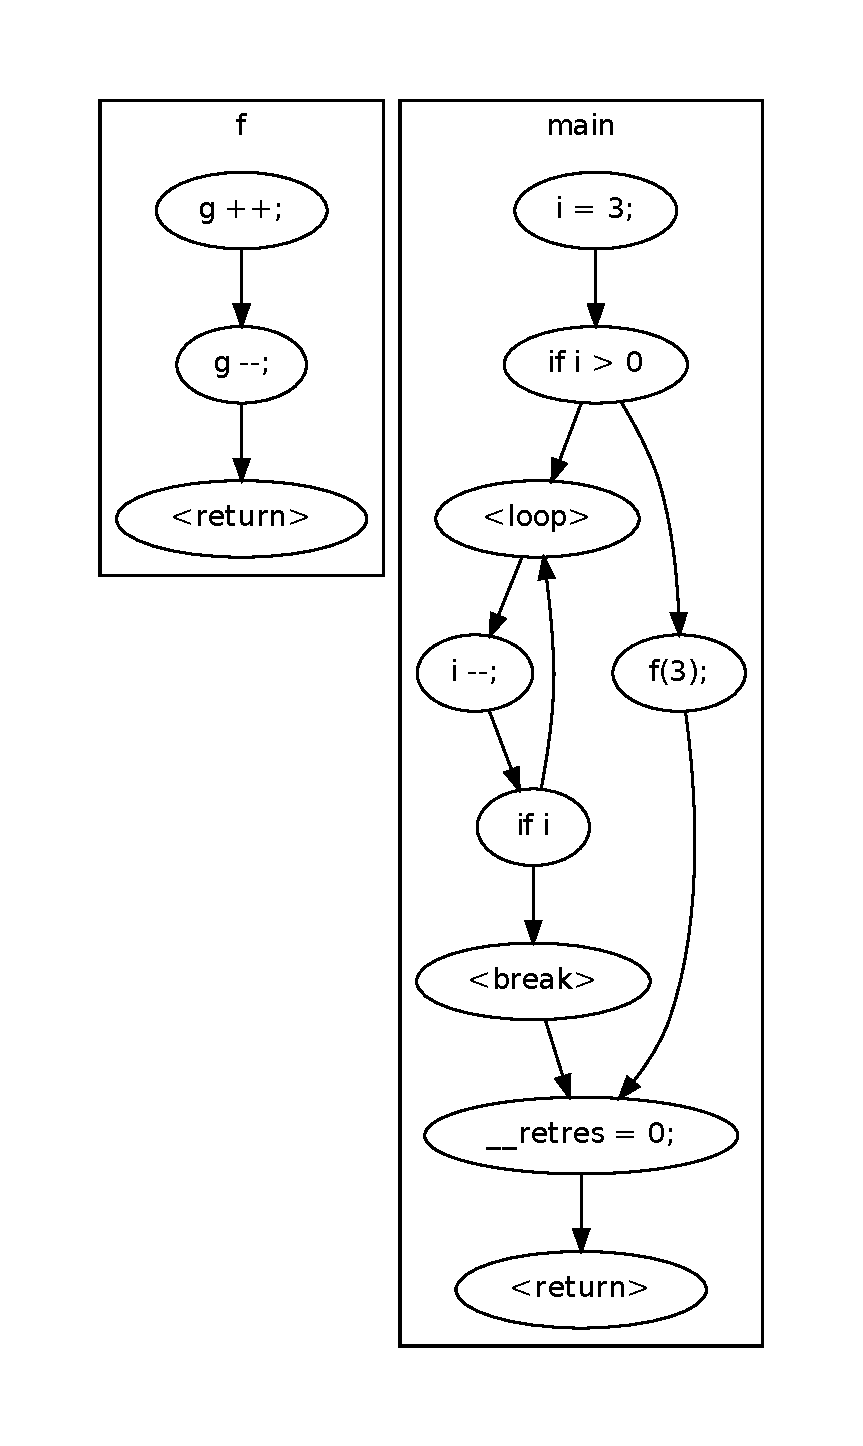
\includegraphics[width=\textwidth]{./tutorial/viewcfg/pdfs/cfg.pdf}
  \end{minipage}

  \caption{Control flow graph for file test.c.}
  \label{fig:tut:basiccfg}
\end{figure}

\subsubsection*{Further improvements}

There are many possible enhancements to this code:

\begin{itemize}
\item There is a bug when trying to print statements that contain
  strings (such as \verb|printf("Hello\n")|, due to double quotes.
  Such statements must be protected using the \verb|"%S"| Format directive;
\item The plug-in could be properly registered as such, allowing it to
  accept command-line options, for instance to compute the control flow graph
  of a single function given as argument;
\item The graphs could be fancier, in particular by distinguishing
  between branching nodes and plain ones, or showing block entries and exits;
  or linking call sites to the called functions.
\end{itemize}

We will concentrate on another extension, which is to reuse the
analysis of the \texttt{Eva} plug-in to color unreachable nodes.
To do so, because we will combine different plug-ins, we need to ensure their
correct ordering. This requires the definition of some command-line options
for our plug-in.

\subsection{Plug-in registration and command-line options}\label{tut2:options}
\index{Plug-in!Command Line Options}\index{Command Line}

We have already seen how to register options in the previous ``Hello'' tutorial.
We now apply these principles to the ViewCfg plug-in.

\ocamlinput[linerange={9-26}]{./tutorial/viewcfg/v2-options/view_cfg.ml}
\scodeidx{Plugin}{Register}
\ocamlinput[linerange={66-74}]{./tutorial/viewcfg/v2-options/view_cfg.ml}
\scodeidx{Visitor}{visitFramacFileSameGlobals}
\scodeidx{Ast}{get}

We added two options, \texttt{-cfg} to compute the CFG
conditionally (important for ordering plug-in executions),
and \texttt{-cfg-output} to choose the output file.

An interesting addition would be a \texttt{-cfg-target} option,
which would take a set of files or functions whose CFG would be
computed, using the \texttt{Self.Kernel\_function\_set} functor. Depending on
the targets, visiting the AST would have different starting points.
This is left as an exercise for the reader.

Another interesting exercise is to solve the following problem.
Currently, the complete CFG for the whole application is computed in
each \framac step, \ie executing \texttt{frama-c test.c -cfg
  -then -report} would compute the CFG twice. Indeed, the
\texttt{-cfg} option sets \texttt{Enabled} to true, and the
\texttt{run} function is executed once per task. To solve this
problem, one has to create a boolean state to remember that the plug-in
has already been executed. The \texttt{apply\_once} function in the
\texttt{State\_builder} module helps dealing with this issue (reading
the section~\ref{tut2:project-and-state} of this tutorial and
section~\ref{adv:project} of this manual should help you understand the
underlying notion of states).

With these command-line options, we can properly interface our ViewCfg plug-in
with the \texttt{eva} plug-in.

\subsection{Interfacing with other plug-ins}

Plug-ins can use functions specified in the public interfaces of other
plug-ins, as long as they are declared as dependencies. To do so, you only
need to add them to the \texttt{libraries} stanza\footnote{A stanza is,
roughly speaking, a ``term'' in \texttt{dune} parlance: a parenthesized
expression.} in the \texttt{dune} file.
We will use a function from the \textsf{Eva} plug-in in our example,
so we will add \texttt{frama-c-eva.core} to the \texttt{dune} file:

\duneinput[linerange={5-5}]{./tutorial/viewcfg/v3-eva/dune}

Now our plug-in can call all functions and access all types declared in
\textsf{Eva}'s public interface.

For historical reasons, several kernel-integrated plug-ins, such as
\textsf{From}, \textsf{InOut} and \textsf{Slicing}, had their API exposed
via the \texttt{Boot} module of the \framac kernel. This has been deprecated
for \textsf{Eva}, and newer plug-ins expose their public interface directly.

In our example, we will use \textsf{Eva}'s new API to obtain reachability
information computed by the value analysis.
The code modification we propose is to color in pink the nodes guaranteed to
be unreachable by the value analysis. For this purpose, we change the
\texttt{vstmt\_aux} method in the visitor:

\ocamlinput[linerange={57-70}]{./tutorial/viewcfg/v3-eva/view_cfg.ml}
\sscodeidx{Eva}{Analysis}{is\_computed}
\sscodeidx{Eva}{Results}{is\_reachable}
\sscodeidx{Cil}{visitAction}{DoChildren}
\sscodeidx{Visitor}{frama\_c\_visitor}{vstmt\_aux}

This code fills the nodes with green if the node may be
reachable, and in pink if the node is guaranteed not to be
reachable; but only if the value analysis was previously computed.

To test this code, we recompile the plug-in with the modified \texttt{dune}
file to take into account the dependency on \textsf{Eva}, as well as the
modified \texttt{vstmt\_aux}. We run \verb|dune build @install| and then
we run \textsf{Eva}, and then our plug-in:
\begin{frama-c-commands}
  dune exec -- frama-c test.c -eva -then -cfg && dotty cfg.dot
\end{frama-c-commands}

The relative order of most options and file names is not important
{\em between} occurrences of \texttt{-then}, but it {\em is} important
whether they are before or after \texttt{-then}-related options
(\texttt{-then}, \texttt{-then-on}, \texttt{-then-last});
see Section~\ref{adv:init} for details. Here, we want to ensure that
\textsf{Eva} is run {\em before} our plug-in, so we order it as
\verb|-eva -then -cfg|. Without \texttt{-then}, even if \texttt{-eva}
is before \texttt{-cfg} in the command line, it is {\em not} guaranteed
that it will run before; options in the same ``block'' can be thought of as
{\em concurrent}: there is no specified order between them.

The resulting graph is shown in Figure~\ref{fig:tut:coloredcfg}.

\begin{figure}[htbp]
  \centering
  \begin{minipage}[h]{0.47\linewidth}
  \listingname{test.c}
  \cinput[linerange={5-999}]{./tutorial/viewcfg/v3-eva/tests/viewcfg/test.c}
  \end{minipage}%
  \begin{minipage}[h]{0.4\linewidth}
    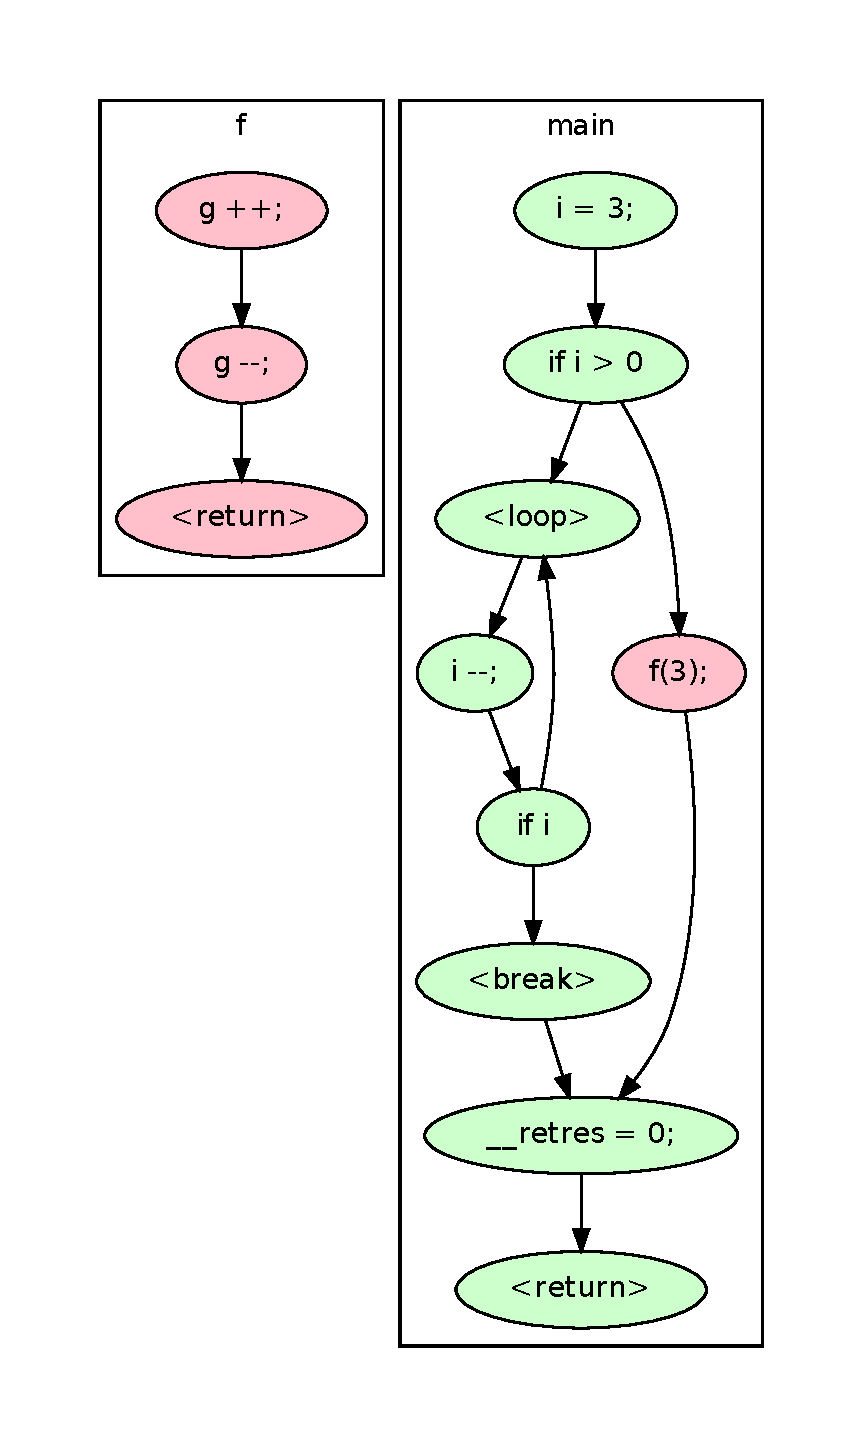
\includegraphics[width=\textwidth]{./tutorial/viewcfg/pdfs/cfg_colored.pdf}
  \end{minipage}
  \caption{Control flow graph colored with reachability information.}
  \label{fig:tut:coloredcfg}
\end{figure}

\subsection{Splitting files and providing a mini-GUI for testing}
\label{tut2:split-and-gui}

Our plug-in is starting to amass enough code that we should envisage to split
it into several modules, for better organizing it. Dune automatically compiles
all source files it finds, unless specified otherwise, and it handles
dependencies between them, so it is essentially free to do so. As we did in the
{\em Hello} tutorial, we will split our \verb|view_cfg.ml| file into smaller
modules.

We will create the following files:

\begin{description}
\item[options.ml]: will contain the module registration (\verb|Self|) and
  command-line options (\verb|Enabled| and \verb|OutputFile|);
\item[visit.ml]: will contain the \verb|print_stmt| function and the visitor;
\item[run.ml]: will contain the definition of function \verb|run| and the
  call to \verb|Boot.Main.extend|.
\end{description}

Note that a few changes are needed to the code: functions from other files
need to include that file name as module, \eg
\verb|Enabled.get| becomes \verb|Options.Enabled.get|.

For simplicity's sake, we will remove options \verb|-cfg| and \verb|-cfg-output|
and replace them with a single boolean option, \verb|-cfg-gui|, to launch the
GUI (this prevents unsuitable combinations of \verb|-cfg| and \verb|-cfg-gui|).
The new option is defined as below:

\ocamlinput[linerange={7-11}]{./tutorial/viewcfg/v4-bogue/options.ml}

And the \verb|run| function in \verb|run.ml| becomes simply:

\ocamlinput[linerange={1-3}]{./tutorial/viewcfg/v4-bogue/run.ml}

We can now erase \verb|view_cfg.ml| and re-run \verb|dune build @install| to
compile the plug-in.

\subsubsection{Mini-GUI for testing}

Extending \framac's Ivette graphical user interface is a task too large for
this tutorial; Ivette being a desktop Electron application, written in
TypeScript and using React, there is a substantial amount of explaining to
do before one can show how to integrate a \framac plug-in in it.

Instead, for this tutorial, we will use a lightweight OCaml GUI library,
BOGUE\footnote{\url{http://sanette.github.io/bogue/Principles.html}}.
You can install it through opam:

\begin{shell}
\$ opam install bogue
\end{shell}

It is based on SDL2, which means you may need to install non-OCaml
dependencies\footnote{With opam $< 2.1$, you may need to install and
run \texttt{depext}. With opam $\geq 2.1$, depext is already included.}.

Since we will be using BOGUE in our plug-in, we need to declare it in the
\texttt{dune} file:

\duneinput[linerange={5-5}]{./tutorial/viewcfg/v4-bogue/dune}

We also need a way to print an individual function as a standalone graph,
without having to call the file visitor (\verb|Visit.vfile|). We will call
it \verb|dump_function| and put it in a separate file, \verb|dump.ml|:

\listingname{./dump.ml}
\ocamlinput{./tutorial/viewcfg/v4-bogue/dump.ml}
\scodeidx{Visitor}{visitFramacFunction}

The code prints a feedback message, then the header, calls the visitor,
and prints the footer. This function will be called by our ``mini-GUI'',
and the output will be sent to \texttt{dotty}, which will open a window
with our graph.

The actual GUI code is put inside a file appropriately named \texttt{gui.ml}:

\listingname{./gui.ml}
\ocamlinput{./tutorial/viewcfg/v4-bogue/gui.ml}
\sscodeidx{Globals}{Functions}{find\_by\_name}
\scodeidx{Kernel\_function}{get\_definition}

Most of the code is boilerplate for Bogue. The only \framac-related part is
the checking of the function name: \verb|Globals.Functions.find_by_name| raises
exception \verb|Not_found| if the name input by the user does not exist. But
even if it does, since we need a function {\em definition}, we must check that
it is not simply {\em declared}. Besides that, we simply call
\verb|dump_function|. Figure~\ref{fig:tut:bogue} shows what this mini-GUI looks
like.

\begin{figure}[htbp]
  \centering
  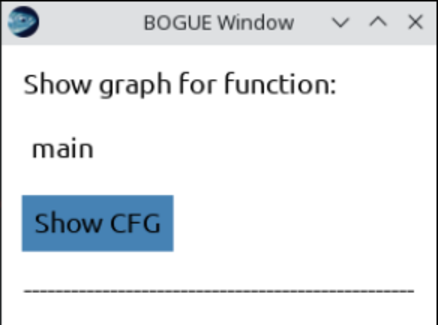
\includegraphics[width=0.35\textwidth]{./tutorial/viewcfg/pdfs/bogue.pdf}
  \caption{Mini-GUI with Bogue for testing our plug-in.}
  \label{fig:tut:bogue}
\end{figure}

Whenever we click the ``Show CFG'' button, a new \texttt{dotty} window is
opened. After we close it, we can repeat the operation as we like.

Note that the feedback message ``Computing CFG for function'' is emitted
each time we click the button, which means we perform a new visit.
For large computations and programs, this is wasteful,
and we should be able to easily cache the result.
The next section will show how to do it using {\em states}.

\subsection{Saving/Loading Data, and Usability in a Multi-Project Setting}
\label{tut2:project-and-state}
\index{Project}

\subsubsection{Registering and using state}

In this section, we will learn how to register state into \framac. A
\emph{state} is a piece of information kept by a plug-in. For instance, we can
use a boolean state to store whether an expensive analysis has been executed,
to avoid recomputing it. Another example of state: the \textsf{Eva} plug-in
computes, for each statement, a table associating to each AST variable a set of
values the program may have at runtime; this association table is a state.

State registration provides several features:
\begin{itemize}
\item It allows the state to be saved and reloaded with the rest of
  the session, for instance when using \texttt{frama-c -save/frama-c
    -load};
\item It helps maintaining consistency between the AST and the results and
  parameters of the analysis of the different plug-ins.
\end{itemize}

We will modify our \verb|Dump| module to output the \dottool graph as a string,
and store it in a hash table from \texttt{fundec} to \texttt{string}.
Storing this string will allow us to memoize~\cite{michie68}
our computation: the string is computed the first time the CFG of a
function is displayed, while the following requests will reuse the result of
the computation. Registering the hash table as a \framac state is
\emph{mandatory} to ensure \framac consistency: for instance, by using a
standard \caml hash table, a user that would have loaded several sessions through
a GUI could observe the CFG of function of a previous session instead of the
one he wants to observe.

Registering a state is done by a functor application:

\ocamlinput[linerange={10-17}]{./tutorial/viewcfg/v5-state/dump.ml}
\scodeidx{State\_builder}{Hashtbl}
\scodeidx{Cil\_datatype}{Fundec}
\scodeidx{Datatype}{String}
\scodeidx{Ast}{self}
\sscodeidx{Eva}{Analysis}{self}

The \texttt{State\_builder} module provides several functors that help
registering states. \texttt{State\_builder.Hashtbl} allows the developer to
create a hash table. It is parameterized by a module describing the hash table
and its key, a module describing the data associated to keys, and
other information.

The \texttt{Datatype} and \texttt{Cil\_datatype} modules describe the
hash table and its associated data, and explain for instance how the
datatype should be copied, printed, or marshalled to the disk. They
are part of the \texttt{Type} library~\cite{signoles:jfla11}, described in
Section~\ref{adv:datatype}. \texttt{Datatype} provides
descriptions for standard \caml types, and \texttt{Cil\_datatype} for
the CIL types (in the \texttt{Cil\_types} module).

The last module argument describes the initial size of the hash table%
\footnote{This initial size is an optimization feature; the table automatically
grows when needed.}, a name (mainly used for internal debugging),
and a list of \emph{dependencies}.
Here we expressed that our hash table depends on the AST and the results of the
\textsf{Eva} plug-in. For instance, whenever the \framac kernel updates one of
these states, it will automatically reset our hash table.
This ensures consistency of the analysis: if the AST of a function changes,
or the value analysis is executed with a different entry point,
this potentially affects the display of the control flow graph,
that we must recompute.

Once the module has been declared, it is fairly easy to use it.

\ocamlinput[linerange={3-8}]{./tutorial/viewcfg/v5-state/dump.ml}
\scodeidx{Visitor}{visitFramacFunction}
\ocamlinput[linerange={19-24}]{./tutorial/viewcfg/v5-state/dump.ml}

\texttt{dump\_function} now takes two steps: first the CFG is printed
to a string, then the string is printed to the \texttt{fmt}
argument. This allows the \texttt{dump\_to\_string} part to be
\emph{memoized}, \ie the results of \texttt{dump\_to\_string} are
saved so that later calls to \texttt{dump\_function} with the same
\texttt{fundec} argument reuse that result.

To check this, we re-run our mini-GUI with:

\begin{frama-c-commands}
\$ dune exec -- frama-c <file> -cfg-gui
\end{frama-c-commands}

The first graph for each function will show the message
``Computing CFG for function ...'', but subsequent calls will no longer do it.

Also, we can see the effects of the dependency on the \textsf{Eva} plug-in
by first launching the value analysis and then our plug-in:

\begin{frama-c-commands}
\$ dune exec -- frama-c <file> -eva -then -cfg-gui
\end{frama-c-commands}

In this case, the graphs will be colored.

Finally, to check that the state dependency on \textsf{Eva} works, we will use
a more complex command line:

\begin{frama-c-commands}
\$ dune exec -- frama-c <file> -eva -then -cfg-gui -then -main f
\end{frama-c-commands}

We have three stages: first run \textsf{Eva}, then open the mini-GUI, then
change the entry point (\verb|-main f| means that the program will start
executing from function \verb|f|) {\em and} re-open the mini-GUI.
Remember that most \framac options {\em persist} from one stage to the next:
the same way that we do not have to repeat \verb|-eva| after the first
\verb|-then|, we do not have to repeat \verb|-cfg-gui| after the second
\verb|-then|. If we want to avoid re-running the mini-GUI in future stages,
we need to use \texttt{apply\_once}, as mentioned in Section~\ref{tut2:options}.

What we observe is the following: when the mini-GUI opens, we click
{\em Show CFG}, see a ``Computing CFG for function ...'' message, and get a
mostly-green CFG. Then, we close the mini-GUI, and it opens again. Clicking
{\em Show CFG} will show the same ``Computing CFG'' message, but the graph will
be entirely pink: with \verb|f| as the entry point, function \verb|main| is
never called, therefore entirely unreachable. Because the entry point changed,
and \textsf{Eva} depends on its state, it is automatically recomputed.
Because our plug-in depends on \textsf{Eva}'s state, it recomputes the graph
when we ask again for the CFG.

Another way to observe how \framac automatically handles states is to display a
CFG, save the session (option \verb|-save <file>|), and then load it again:

\begin{frama-c-commands}
\$ dune exec -- frama-c <file> -eva -then -cfg-gui -save session.sav
\end{frama-c-commands}

Then click on the ``Show CFG'' (see the feedback message), then close the CFG
and the mini-GUI. Reload the session:

\begin{frama-c-commands}
\$ dune exec -- frama-c -load session.sav
\end{frama-c-commands}

Click ``Show CFG'' and you will {\em not} see the ``Computing CFG'' message:
the state \texttt{Cfg\_graph\_state} had beem automatically saved by \framac
and has just been loaded from the session.

\subsubsection{Clearing states, selection and projects}

There is one caveat though: if the user computes the CFG before
running the \textsf{Eva} analysis, and then runs \textsf{Eva}, they
will not see a colored graph (unless they re-launch \textsf{Eva}
with different parameters). This is because the state of the
CFG is reset when the state of \textsf{Eva} is reset, not when it is
first computed.

To solve this problem, we will manually reset the
\texttt{Cfg\_graph\_state} if we detect that \textsf{Eva}
has been run since the last time we computed the CFG. For
that, we have to remember the previous value of
\texttt{Eva.Analysis.is\_computed ()}, \ie to register another state:

\ocamlinput[linerange={19-25}]{./tutorial/viewcfg/v6-state-clear/dump.ml}
\scodeidx{State\_builder}{Ref}
\scodeidx{Datatype}{Bool}

This new state only consists of a reference to a boolean value.

Then we just replace \texttt{dump\_function} in the code above by the
following.

\ocamlinput[linerange={29-37}]{./tutorial/viewcfg/v6-state-clear/dump.ml}
\sscodeidx{Eva}{Analysis}{is\_computed}
\sscodeidx{State\_selection}{S}{with\_dependencies}
\scodeidx{Project}{clear}

The only parts that need to be explained are the notions of
\emph{selection} and \emph{project}. A selection is just a set of
states; here we selected the state \texttt{Cfg\_graph\_state} with all
of its dependencies, as resetting this state would also impact states
that would depend on it (even if there are none for now). We use
\texttt{Project.clear} to reset the selection.

\subsubsection{Project explanation}

A \emph{project}~\cite{project} is a consistent version of all the \emph{states}
of \framac. \framac is multi-AST, \ie \framac plug-ins can change the AST of the
program, or perform incompatible analyses (\eg with different entry
points). Projects consistently group a version of the program's AST with
the states related to it.

The \texttt{Project.clear} function has type:
\begin{ocamlcode}
val clear: ?selection:State_selection.t -> ?project:t -> unit -> unit
\end{ocamlcode}
\scodeidxdef{Project}{clear}
\scodeidx{State\_selection}{t}
\codeidx{Project}
\sscodeidx{Datatype}{Ty}{t}

The arguments \texttt{selection} and \texttt{project} can be seen as a
coordinate system, and the function allows to clear specific versions
of specific states. By default, \framac functions act on the
\emph{current} project. The developer has to use \texttt{Project.on} or optional
arguments to act on different projects. \framac automatically handles
duplication and switch of states when duplicating or changing of
projects. This is the last benefit of state registration.

To summarize:

\begin{itemize}
\item To store results, plug-ins should register \emph{states};
\item A \emph{project} is a consistent version of all the states in
  \framac, together with a version of the AST;
\item A \emph{session} is a set of \emph{projects};
\item \framac transparently handles the versioning of states when
  changing or duplicating projects, saving and reloading sessions from
  disk, etc.
\item The version of the state in a project can change; by default
  \framac functions operate on the current project.
\item A \emph{selection} is a set of states. \emph{Dependencies} allow
  to create selections.
\item As a plug-in developer, you have to remember that is up to you to preserve
  consistency between your states and their dependencies by clearing the latter
  when the former is modified in an incompatible way. For instance, it would
  have been incorrect not to call
  \texttt{State\_selection.with\_dependencies}
  \sscodeidx{State\_selection}{S}{with\_dependencies}
  in the last code snippet of this tutorial.
\end{itemize}

Projects are generally created using copy visitors. We encourage the reader to
experiment with multi-project development by using them. An interesting
exercise would be to change the AST so that execution of each instruction is
logged to a file, and then re-read that file to print in the CFG how many times
each instruction has been executed. Another interesting exercise would be
to use the \texttt{apply\_once} function so that the ViewCfg plug-in is executed
only once, as explained in section~\ref{tut2:options} of this tutorial.
